\chapter{Collective Disambiguation of Named Entities}
\section{The key intuition}
We have seen several different ``local'' solutions, attempting to solve the problem by collecting evidence
around a mention and then using it to disambiguate. Milne and Witten [\ref{mw}] 
came close to inculcating some sort of coherence, but they couldn't totally build up the intuition. It was after a wait of 2 years that CSAW [\ref{thepaper}] took the game 
to a whole new level by working on the following key intuition :	
\begin{itemize}
  \item A document is usually about one topic \bigskip
  \item Disambiguating each entity using the local clues misses out on a major piece of information : Topic of a page \bigskip
  \item A page is usually has one topic, you can expect all the entities to be \emph{related} to the topic \emph{somehow} \bigskip
  \end{itemize}
  \textcolor{green}{Michael Jackson} : 30 Disambiguations 
  
 \textcolor{green}{John Paul} : 10 disambiguations 
 
 
 
  But if they are mentioned on the \textbf{same page}, the page is most likely about Christianity,
  A big hint towards disambiguating \textbf{both} of them.
  
Since the CSAW[\ref{thepaper}] paper, every work on named entity disambiguation includes a 
notion of \emph{Topical coherence} in the solution. 

\section{Challenges}
Though the notion of topical coherence is very natural and intuitive, there are 
a lot of challenges involved when it comes to actually mapping these intuitions to an optimization
problem.
We present the challenges involved and the solution given by the CSAW team.
 \begin{itemize}
  \item Capturing local compatibility
  \begin{itemize}
   \item \textcolor{blue}{Create a scoring function to rank possible candidates}
  \end{itemize}

  \item Inculcating topical coherence in the overall objective

  \begin{itemize}
   \item \textcolor{blue}{Define Topical coherence}
  \end{itemize}

  \end{itemize}

 Out of these two challenges, various solutions to the problem of capturing the local compatibility are presented in Chapter 2. 
 In this chapter, we focus on the problem of collective disambiguation. 
 
 \section{The Dominant Topic Model}
  \begin{itemize}
   \item Need to define a collective score based on pairwise topical coherence of all $\gamma_s$ used for labeling. \medskip
   \item The pairwise topical coherence, $r(\gamma_s, \gamma_s')$ is as defined above.\medskip
   \item For a page, overall topical coherence : \begin{center}\medskip
                                                  $\Sigma_{s \neq s' \in S_0}r(\gamma_s, \gamma_s')$
                                                 \end{center}
   \item Can be written as clique potential as in case of node potential\medskip
      \begin{center}
	$exp(\Sigma_{s \neq s' \in S_0}r(\gamma_s, \gamma_s'))$
      \end{center}

  \end{itemize}

  \section{The Optimization objective}
  With different notations as above, we would like to maximize the following to get the 
  best results.
 \begin{center}
 $\frac{1}{\binom{|S_0|}{2}}\Sigma_{s \neq s' \in S_0}r(\gamma_s, \gamma_s') + \frac{1}{|S_0|}\Sigma_{s \in S_0}w^{T}f_s(\gamma)$
  \\
  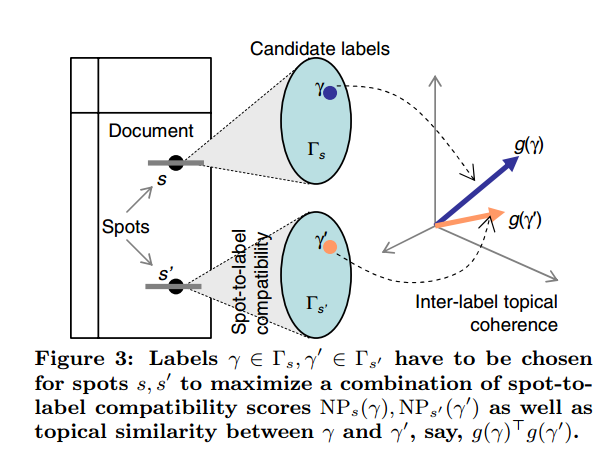
\includegraphics[height = 5 cm]{objective}\footnote{From \ref{thepaper}}
  \end{center}
  In verbose, we want that the entity-entity coherence be maximized, while choosing the disambiguation which is the best.

 
  \section{Solving the optimization objective}
  The authors compare 2 different approaches for solving the optimization objective.
  \begin{itemize}
   \item LP rounding approach\bigskip
   
    $|\Gamma|$ + $|\Gamma|^2$ binary variables were introduced. The first set of binary variables decide the candidate that
   each mention takes, and the second set has one binary variable for each possible candidate pair. 
   The authors relax this integer programming to a linear programming and then used rounding with a threshold of 0.5 to
   obtain the best solution.
   
   \item Hill climbing
   
   Starting from all assignments set to NA, assignments are done based on local potentials only. The following figure (
   from the paper) illustrates the process.
   \begin{center}
    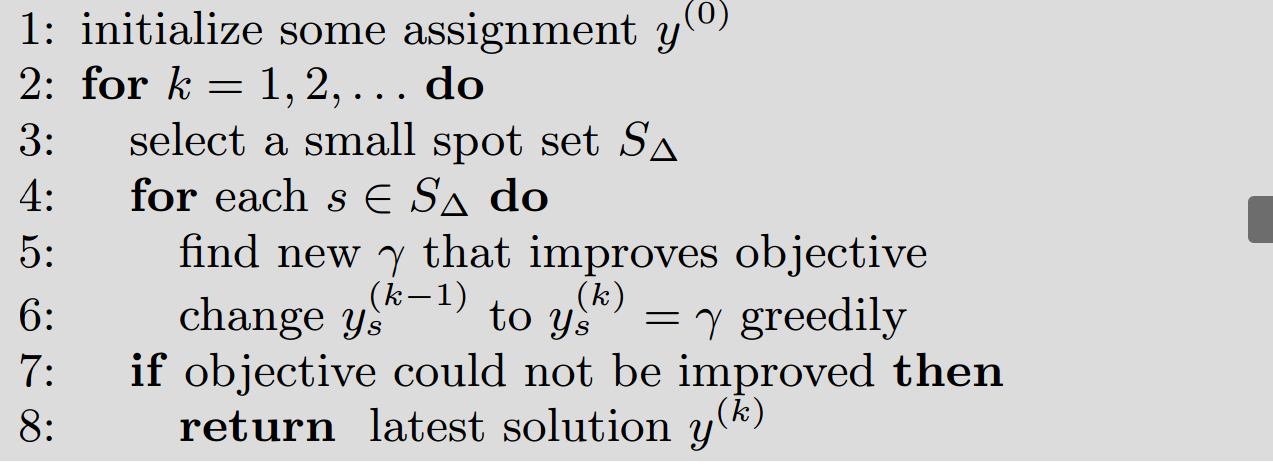
\includegraphics[height = 3cm]{hill}
   \end{center}

  \end{itemize}


\chapter{Pragmatic combination of Local and Global Disambiguations}

\section{Introduction}

Recall that Chapter 2 was about local disambiguation. In chapter 3, we saw how
global disambiguation can be combined with the overall objective. A recent work, 
Robust disambiguation of named entities in text [\ref{aida}], proposes that 
blindly opting for global disambiguation may not be always right. 
Consider the sentence : ``Manchester will play Madrid in Barcelona''.

All the 3 named entities in the sentence are Cities as well as football clubs.
Collective disambiguation may \emph{coerce} all the three mentions to be 
either football clubs or cities. The work aims to solve this problem by being selective about when to go for collective disambiguation.

\section{Approach}
This approach first creates a mention to candidate graph. The sample graph for the sentence ``They performed Kashmir 
written by Page and Plant. Page played unusual chord on his Gibson.'' is as shown below : 
 \begin{figure}[H]
 \centering
 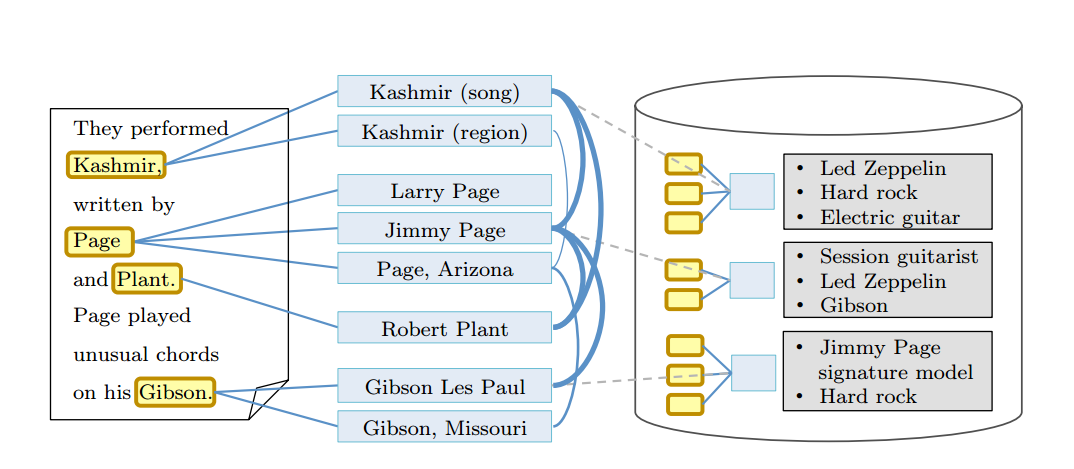
\includegraphics[bb=0 0 1074 469,scale=0.3]{./megraph.png}
 % megraph.png: 1074x469 pixel, 72dpi, 37.88x16.54 cm, bb=0 0 1074 469
 \caption{Mention Entity Graph}
\end{figure}


Having created the graph, we need to assign the edge weights. Clearly, there are 2 kinds of edges involved : 
\begin{itemize}
 \item Mention - Entity edge : The authors used a knowledge based approach to assign this weight. This is as outlined in chapter 2.
 The details about this score are given in [\ref{kpsim}].
 \item Entity - Entity edge : Milne witten score as defined in chapter 2 is used for this purpose.
\end{itemize}

With the graph ready, the authors pluck the in a greedy manner such that there is only one edge between each 
mention and entity.


\chapter{Further Readings on Named Entity Disambiguation}

For this report, only a small subset of the papers was selected to cover as much ground as possible.
The following list may be valuable to the interested readers.

\begin{itemize}
\item \textbf{Mining evidences for named entity disambiguation}
The authors discuss a modified LDA model for gathering more words that are important to disambiguate an entity. 
Li, Yang, et al. "Mining evidences for named entity disambiguation." Proceedings of the 19th ACM SIGKDD international conference on Knowledge discovery and data mining. ACM, 2013.
 \item \textbf{We have emphasized on Wikipedia as the catalog. The following work presents a general approach} \\
 Sil, Avirup, et al. "Linking named entities to any database." Proceedings of the 2012 Joint Conference on Empirical Methods in Natural Language Processing and Computational Natural Language Learning. Association for Computational Linguistics, 2012.
 \item \textbf{Large scale named entity disambiguation.} \\
 Cucerzan, Silviu. ``Large-Scale Named Entity Disambiguation Based on Wikipedia Data.'' EMNLP-CoNLL. Vol. 7. 2007.
 \item \textbf{One of the initial works on NED} \\
 Bunescu, Razvan C., and Marius Pasca. "Using Encyclopedic Knowledge for Named entity Disambiguation." EACL. Vol. 6. 2006.
 \item \textbf{Quick entity annotations for short text} \\
 Suchanek, Fabian M., Gjergji Kasneci, and Gerhard Weikum. "Yago: a core of semantic knowledge." Proceedings of the 16th international conference on World Wide Web. ACM, 2007.
\end{itemize}
